\section{Evaluatie}
\label{sec:eva}

\subsection{Resultaten}

\subsubsection{Deelvraag 1}
Het beste resultaat werd bereikt met SVM gebruikmakend van \textit{stochastic gradient descent learning}
%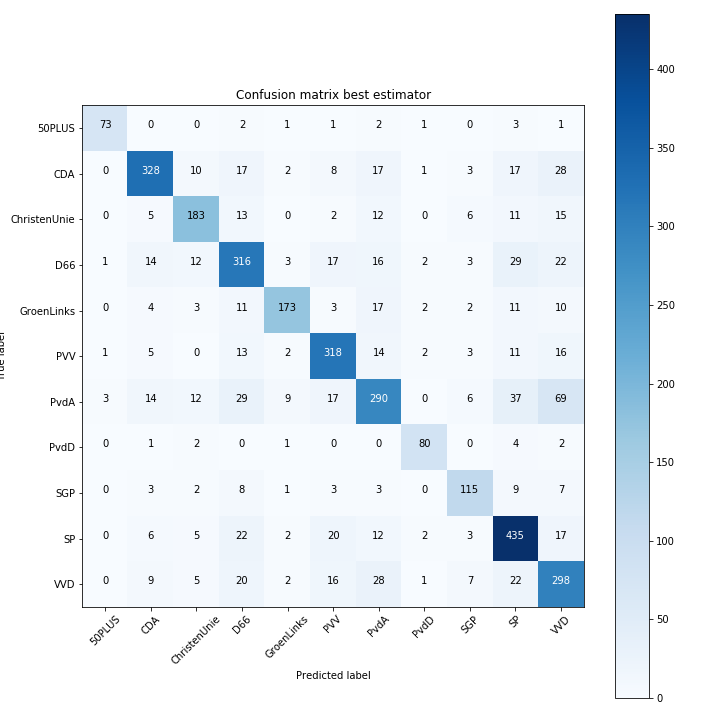
\includegraphics[width=0.6\paperwidth]{Verslag/confusionmatrix.png}

\begin{figure}
  \caption{Confusion matrix van beste classificatie.}
  \centering
    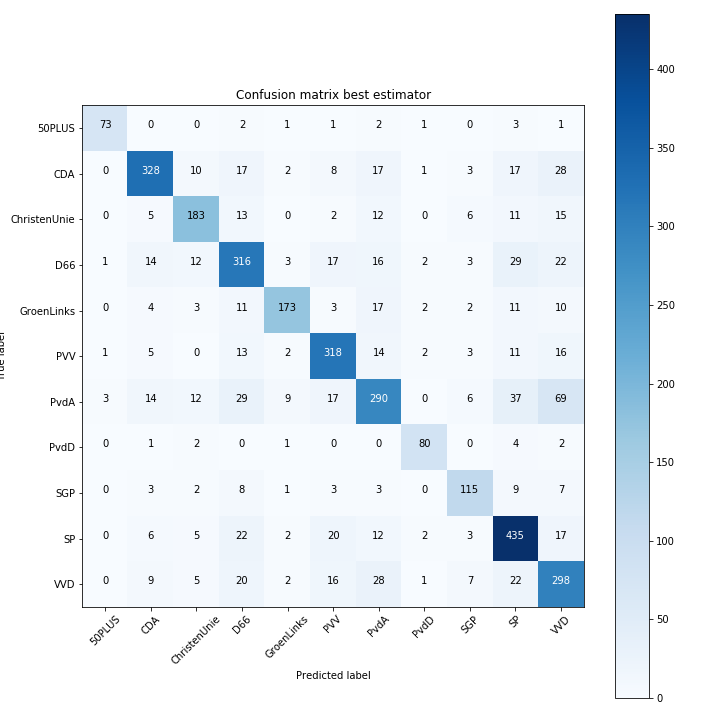
\includegraphics[width=0.6\paperwidth]{Verslag/confusionmatrix.png}
\end{figure}

\subsubsection{Deelvraag 2}
\begin{table}[H]
\label{aantallen}
\caption{Meest relevante woorden per partij op basis van beste classifier}
\centering
\begin{tabular}{llllllllllll}
\toprule
0 &        gepensioneerd &             yyyyy &  voedselverspill &  mijn fractie &                 schon &       islamitisch &             de yyyyy &              dier &  mevrouw de voorzitter &        huurder &          de yyyyy \\
1 &                ouder &           inwoner &           gezinn &          mijn &      belastingontwijk &           miljard &               kinder &            milieu &               dank zer &  geheim dienst &       de yyyyy is \\
2 &           50 plusser &  de yyyyy fractie &   fractie van de &        vandag &         schon energie &         nederland &            circulair &         industrie &                   punt &     segregatie &      vor de yyyyy \\
3 &              plusser &     yyyyy fractie &      prostitutie &         natur &     kamer hierover te &          de yyyyy &  voorzitter de yyyyy &               bio &             mevrouw de &     bestuurder &  de yyyyy betreft \\
4 &  koopkrachtontwikkel &             reger &     mensenhandel &         yyyyy &          in elk geval &           brussel &               jonger &            de bio &               allerlei &           zegt &              huis \\
5 &                yyyyy &          de reger &            motie &       fractie &                   zou &          de islam &           lager over &     bio industrie &               de yyyyy &         armoed &          regelgev \\
6 &       ouderenwerklos &              eran &       rechtsstat &   buitengewon &             elk geval &             islam &           ieder kind &   klimaatverander &             beantwoord &      de bevolk &      wat de yyyyy \\
7 &                   50 &              hier &         inderdad &       hervorm &  hierover te informer &  belastingbetaler &          mijn partij &  de bio industrie &            bewindslied &           mens &            veilig \\
8 &    fractie van yyyyy &          antwoord &         rookvrij &        daarom &              vluchtel &       asielzoeker &                  hun &            burger &      vor de beantwoord &         bevolk &         speelveld \\
9 &              werkend &         vor yyyyy &             zull &      minister &           hierover te &           mijnher &         arbeidsmarkt &     constater dat &          de beantwoord &      voorstell &       bedrijfslev \\
\bottomrule
\end{tabular}

\end{table}

\subsection{Discussie}
\subsubsection{Deelvraag 1}
Dit onderzoek heeft zich beperkt tot methoden genoemd in vergelijkbare onderzoeken én waarvan de implementatie beschikbaar is in Python. Een aantal methoden die in gerelateerde literatuur leidden tot goede classificaties zijn daarom niet getest. Ook nieuwe methoden die nog niet gebruikt zijn in een vergelijkbaar onderzoek voor politieke tekst classificatie zijn daarom niet getest. Omdat dus niet alle opties getest zijn, kan geen uitsluitsel gegeven worden dat dit daadwerkelijk het classificatiemodel is. Voor vervolgonderzoek kan daarom gekeken worden naar meer verschillende methoden.\par



\subsubsection{Deelvraag 4}
Er zijn verschillende visies op links en rechts, en de indeling van de partijen, ook buiten de twee methoden gekozen in dit onderzoek.\par